\chapter{Thread}
Fino ad ora abbiamo visto dei processi in esecuzione che possono alternarsi oppure essere in esecuzione contemporanea in base al numero di processori che si trovano sulla macchina. Tuttavia, per alcune applicazioni è importante essere organizzate in modo parallelo ed è il programmatore stesso a suddividere l'applicazione in diverse esecuzioni, ciascuna esecuzione si chiama \textit{thread}. Un esempio tipico di thread è un'applicazione grafica.

Diversi thread di uno stesso processo condividono tutte le risorse (memoria, file, dispositivi di I/O...) tranne lo stack delle chiamate e il processore.

\textit{Ma quali sono i vantaggi di utilizzare i thread che non possono essere soddisfatti attraverso il solo utilizzo alternato o parallelo dei processi?} In verità utilizzare i thread, come vedremo, è più semplice ed efficiente per la creazione, terminazione, switching e comunicazione tra thread.

\section{Processi e thread}
Si può dire quindi che il concetto di processo incorpora due caratteristiche: gestione delle risorse, dove i processi vanno intesi come blocco unico, e scheduling/esecuzione, dove i processi possono contenere diverse tracce (thread).

\begin{figure}[h]
    \centering
    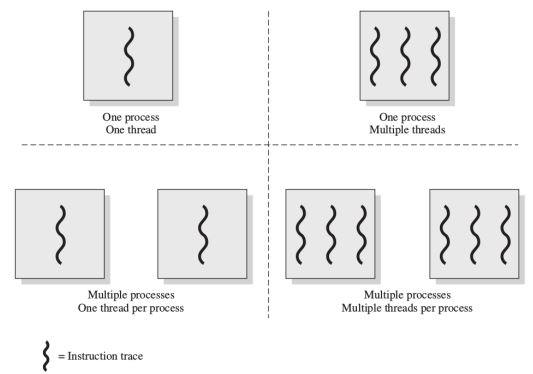
\includegraphics[width=0.5\linewidth]{images/processi-e-thread1.JPG}
    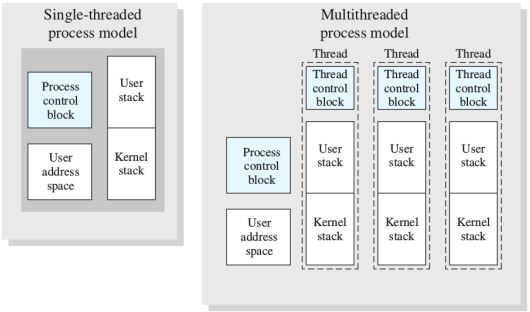
\includegraphics[width=0.49\linewidth]{images/processi-e-thread2.JPG}
    \caption{Gestione dei processi e thread}
    \label{fig:processi-e-thread}
\end{figure}

In base al numero di processi in esecuzione possiamo trovare, nel sistema operativo, uno o più thread per processo. In entrambe i casi rimangono il PCB e l'indirizzo o immagine comune a tutti i thread, mentre, nel multithread, ogni thread viene gestito attraverso un \textit{Thread control block} per lo scheduling, uno stack delle chiamate utente e uno stack per le chiamate di sistema.\\\\
Ogni processo viene creato con un thread, dopodiché il programmatore può eseguire un'opportuna chiamata di sistema che: genera un nuovo thread (\textit{spawn}); blocca un thread (\textit{block}); sblocca un thread (\textit{unblock}); termina un thread (\textit{finish}).

\section{Tipi di thread}
E' necessaria una distinzione tra thread a livello utente (\textit{User Level Thread - ULT}) e thread a livello di sistema (\textit{Kernel Level Thread - KLT}).

\begin{figure}[h]
    \centering
    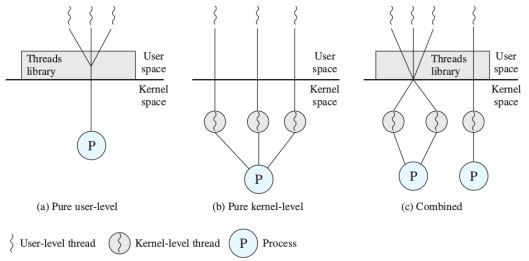
\includegraphics[width=0.7\linewidth]{images/ult-klt.JPG}
    \caption{User Level Thread e Kernel Level Thread}
    \label{fig:ult-klt}
\end{figure}

Nei primi, il sistema operativo vede solo un processo, e non ha nessuna idea che al suo interno è diviso in thread, perché ci sono delle opportune librerie (\textit{Threads library}) che gestiscono direttamente i thread del processo. Con i KLT, invece, il sistema operativo è a conoscenza della divisione in thread del processo e le librerie di thread si utilizzano direttamente le system call del sistema operativo.

Con gli ULT: è più facile ed efficiente lo switch; si può avere una politica di scheduling diversa per ogni applicazione; permettono di usare i thread anche sui sistemi operativi che non li offrono nativamente. Ma allo stesso tempo: se un thread si blocca, si bloccano tutti i thread di quel processo; se ci sono effettivamente più processori o più cores, tutti i thread del processo ne possono usare uno solo; se il sistema operativo non ha i KLT, non si possono utilizzare thread per le routine del sistema operativo stesso.

\section{Processi e thread in Linux}
In Linux l'unità di base sono i thread che vengono chiamati LWP (\textit{Lightweight process}). Sono presenti sia gli ULT che i KLT ma vengono utilizzati in maniera diversa: i KLT vengono usati principalmente dal sistema operativo e qualsiasi utente può scrivere degli ULT, che vengono poi mappati in KLT (pthreads). Ad ogni thread, inoltre, viene associato un PID unico che lo identifica e un suo PCB. L'entry del PCB che dà il PID comune a tutti i thread di un processo è il TGID (\textit{Thread Group Identifier}) che coincide con il primo thread del processo.
\begin{figure}[h]
    \centering
    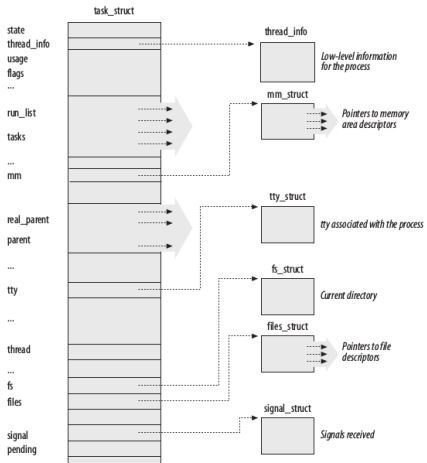
\includegraphics[width=0.5\linewidth]{images/pcb-linux.JPG}
    \caption{PCB in Linux}
    \label{fig:pcb-linux}
\end{figure}
Nel PCB di Linux, la struttura \textit{thread\_info} è organizzata anche per contenere il kernel stack, ovvero, lo stack delle chiamate da usare quando il processo passa in modalità sistema. Il \textit{thread\_group} punta agli altri thread di questo stesso processo e \textit{parent} e \textit{real\_parent} puntano al padre del processo, ci sono anche link per i fratelli e i figli.

Lo schema degli stati in Linux è come quello a 5 stati (vedi Figura \ref{fig:stati-dei-processi}) ovvero, non fa un'esplicita menzione a processi suspended. Tuttavia, internamente il kernel usa questi stati: \textit{Task Running}: include sia Ready che Running; \textit{Task interruptible, Task uninterruptible, Task stopped, Task traced}: sono tutti Blocked, la differenza la fa il motivo per cui sono blocked; \textit{Exit Zombie, Exit Dead}: sono entrambi Exit.

\subsection*{Segnali e interrupt in Linux}
Non bisogna confondere segnali con interrupt (o eccezioni): i segnali possono essere inviati da un processo ad un altro tramite system call. Quando ciò succede, il segnale appena lanciato viene aggiunto all'opportuno campo del PCB del processo ricevente e, quando il processo viene nuovamente schedulato per l'esecuzione, il kernel controlla prima se ci sono segnali pendenti e nel caso esegue un'opportuna funzione chiamata \textit{signal handler}.

\begin{Example}{Segnali e interrupt in Linux}{}
    \textit{Si esegue un programma C scritto male, che accede ad una zona di memoria senza averla prima richiesta.}

    Il processore fa scattare un'eccezione e viene eseguito l'opportuno exception handler (in kernel mode), che essenzialmente manda il segnale \verb|SIGSEGV| al processo colpevole. Quando il processo colpevole verrà selezionato nuovamente per andare in esecuzione, il kernel vedrà dal PCB che c'è un segnale pendente, e farà in modo che venga eseguita l'azione corrispondente. L'azione di default per tale segnale è: fai terminare il processo, ma può essere riscritta dall'utente.
\end{Example}